% Build from this directory:
% latex -interaction=nonstopmode -halt-on-error pam-4.tex
% dvisvgm --no-fonts --exact --bbox=papersize pam-4.dvi -o pam-4.svg
\documentclass[tikz,border=4pt]{standalone}
\begin{document}
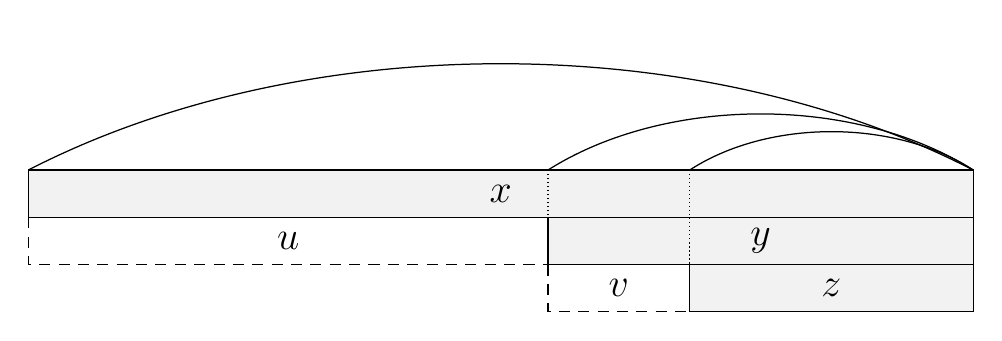
\begin{tikzpicture}[line width=0.45pt,font=\fontsize{14}{17}\selectfont,
  part/.style={fill=black!5},omitted/.style={dash pattern=on 4pt off 3pt}]
  % Right-aligned palindromes: x = uy and y = vz.
  \draw[part] (0,0) rectangle (12,-0.6);
  \draw[part] (6.6,-0.6) rectangle (12,-1.2);
  \draw[part] (8.4,-1.2) rectangle (12,-1.8);
  \draw[omitted] (0,-0.6) -- (0,-1.2) -- (6.6,-1.2);
  \draw[omitted] (6.6,-1.2) -- (6.6,-1.8) -- (8.4,-1.8);
  \draw[densely dotted] (6.6,0) -- (6.6,-0.6);
  \draw[densely dotted] (8.4,0) -- (8.4,-1.2);
  % The arcs show the three nested palindromic suffixes.
  \draw (0,0) .. controls (3.5,1.8) and (8.5,1.8) .. (12,0);
  \draw (6.6,0) .. controls (8.1,0.95) and (10.5,0.95) .. (12,0);
  \draw (8.4,0) .. controls (9.4,0.65) and (11,0.65) .. (12,0);
  \node at (6,-0.3) {$x$};
  \node at (3.3,-0.9) {$u$};
  \node at (9.3,-0.9) {$y$};
  \node at (7.5,-1.5) {$v$};
  \node at (10.2,-1.5) {$z$};
\end{tikzpicture}
\end{document}
